\documentclass[10pt,aspectratio=169]{beamer}

\usepackage[english]{babel}
\usepackage{amsmath}
\usepackage{booktabs}
\usepackage{graphicx}
\usepackage{tabularx}
\usepackage{tikz}
\usetikzlibrary{arrows.meta,positioning,calc,shapes.geometric}

\usetheme{metropolis}
\metroset{progressbar=frametitle,block=fill,numbering=fraction}

\definecolor{themecolor}{RGB}{0,116,178}
\definecolor{riskcolor}{RGB}{40,120,168}
\definecolor{moralitycolor}{RGB}{91,140,90}
\definecolor{actioncolor}{RGB}{148,103,168}
\definecolor{goodcolor}{RGB}{57,122,88}
\definecolor{warncolor}{RGB}{194,107,57}
\definecolor{lightblue}{RGB}{231,241,247}
\definecolor{lightgreen}{RGB}{232,241,232}
\definecolor{lightorange}{RGB}{249,237,228}
\definecolor{lightgray}{RGB}{241,241,239}

\setbeamercolor{title}{fg=themecolor}
\setbeamercolor{structure}{fg=themecolor}
\setbeamercolor{frametitle}{fg=white,bg=themecolor}
\setbeamercolor{background canvas}{bg=white}
\setbeamercolor{alerted text}{fg=warncolor}
\setbeamersize{text margin left=7mm,text margin right=7mm}
\setbeamerfont{caption}{size=\scriptsize}

\graphicspath{{../../results/phase4/LW01/}%
  {../../results/phase4/LW01/presentation/}%
  {../../results/phase5/LW01/presentation/}}

\newcommand{\source}[1]{\vfill{\tiny\color{gray}#1}}
\newcommand{\pill}[2]{%
  \tikz[baseline=(text.base)]\node[rounded corners=2pt,fill=#1!15,
  text=#1,inner xsep=5pt,inner ysep=2pt] (text) {\scriptsize\bfseries #2};}
\newcommand{\fullslide}[1]{%
  \begin{frame}[plain]
    \begin{tikzpicture}[remember picture,overlay]
      \node at (current page.center)
        {\includegraphics[width=\paperwidth,height=\paperheight]{#1}};
    \end{tikzpicture}
  \end{frame}}

\tikzset{
  flowbox/.style={draw=themecolor,fill=lightblue,rounded corners=3pt,
    minimum width=2.15cm,minimum height=0.78cm,align=center,font=\small\bfseries},
  smallflow/.style={draw=themecolor,fill=lightblue,rounded corners=3pt,
    minimum width=1.8cm,minimum height=0.68cm,align=center,font=\scriptsize\bfseries},
  flowarrow/.style={-{Latex[length=2.2mm]},thick,draw=themecolor},
  graphnode/.style={circle,draw=themecolor,fill=lightblue,minimum size=8mm,
    inner sep=0pt,font=\small\bfseries},
}

\title{From Gamebook Graphs to Narrative Experience}
\subtitle{A profile-dependent Bag-of-Paths model enriched with local LLMs}
\author{Guillaume Guex}
\institute{University of Lausanne}
\date{}

\begin{document}

% Slide 1
\begin{frame}[plain]
  \vfill
  {\usebeamerfont{title}\color{themecolor}\inserttitle\par}
  \vspace{3mm}
  {\usebeamerfont{subtitle}\color{themecolor}\insertsubtitle\par}
  \vspace{4mm}
  {\color{warncolor}\rule{0.80\textwidth}{1.2pt}\par}
  \vspace{6mm}
  {\small\insertauthor\par}
  \vspace{2mm}
  {\scriptsize\insertinstitute\par}
  \vspace{7mm}
  {\small\color{gray}
    Can structural differences between player profiles become perceptible
    differences between complete stories?\par}
  \vfill
\end{frame}

% Slide 2
\begin{frame}{A graph captures choices---but loses their meaning}
  \begin{columns}[T,onlytextwidth]
    \column{0.52\textwidth}
      \begin{block}{Paragraph 30}
        \small
        A wagon carrying small children breaks down as a Kraan approaches.
        The children scream in panic.
      \end{block}

      \vspace{2mm}
      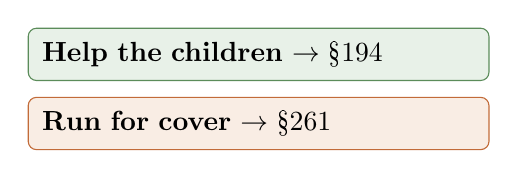
\begin{tikzpicture}[node distance=2mm]
        \node[draw=moralitycolor,fill=lightgreen,rounded corners=3pt,
          text width=5.5cm,align=left,inner sep=5pt] (help)
          {\textbf{Help the children} $\rightarrow$ \S194};
        \node[below=of help,draw=warncolor,fill=lightorange,rounded corners=3pt,
          text width=5.5cm,align=left,inner sep=5pt] (run)
          {\textbf{Run for cover} $\rightarrow$ \S261};
      \end{tikzpicture}

      \vspace{2mm}
      \small A conventional graph records two outgoing edges, but not what
      distinguishes them as actions.

    \column{0.44\textwidth}
      \centering
      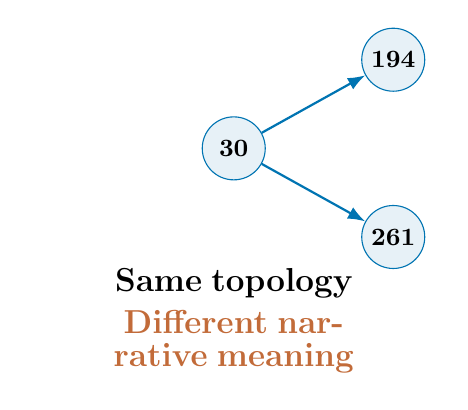
\begin{tikzpicture}[node distance=1.55cm]
        \node[graphnode] (p30) {30};
        \node[graphnode,above right=0.55cm and 1.45cm of p30] (p194) {194};
        \node[graphnode,below right=0.55cm and 1.45cm of p30] (p261) {261};
        \draw[flowarrow] (p30) -- (p194);
        \draw[flowarrow] (p30) -- (p261);
        \node[below=1.0cm of p30,align=center,text width=5cm]
          {\large\bfseries Same topology\\[1mm]
           \color{warncolor}Different narrative meaning};
      \end{tikzpicture}
  \end{columns}

  \source{Example from Joe Dever, \emph{Flight from the Dark}, \S30.}
\end{frame}

% Slide 3
\begin{frame}{Lone Wolf 1 as a controlled case study}
  \centering
  \small\textbf{350 narrative sections} \quad $\bullet$ \quad choices, Kai disciplines,
  combat, inventory, endurance and chance

  \vspace{2mm}
  \begin{columns}[T,onlytextwidth]
    \column{0.315\textwidth}
      \begin{block}{Semantically modelled}
        \footnotesize
        \textcolor{riskcolor}{\textbf{Risk}}\\
        cautious / neutral / reckless

        \smallskip
        \textcolor{moralitycolor}{\textbf{Morality}}\\
        selfish / neutral / noble

        \smallskip
        \textcolor{actioncolor}{\textbf{Action}}\\
        physical / neutral / tactical
      \end{block}

    \column{0.33\textwidth}
      \begin{block}{Fixed-probability assumptions}
        \footnotesize
        Combat win: \textbf{0.833}\\[1mm]
        Kai available: \textbf{0.5}\\[1mm]
        Escape available: \textbf{0.5}\\[1mm]
        \texttt{has\_condition}: \textbf{0.5}

        \smallskip
        Values are experimental parameters, not player-profile dimensions.
      \end{block}

    \column{0.315\textwidth}
      \begin{block}{Not dynamically simulated}
        \footnotesize
        Detailed inventory state\\[1mm]
        Gold and object histories\\[1mm]
        Changing endurance\\[1mm]
        Combat difficulty over time

        \smallskip
        These remain explicit limits of the present model.
      \end{block}
  \end{columns}

  \vspace{1mm}
  \small\color{warncolor}\textbf{Modelling boundary:}
  the aim is a transparent experimental abstraction---not a complete game engine.
\end{frame}

% Slide 4
\begin{frame}{An auditable pipeline from text to trajectories}
  \centering
  \resizebox{0.98\textwidth}{!}{%
  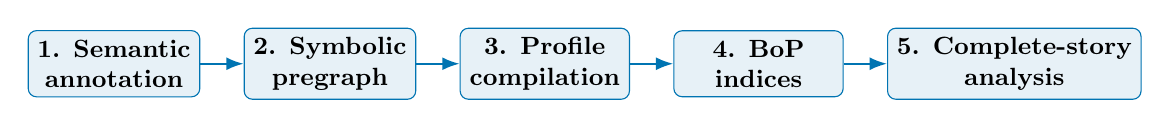
\begin{tikzpicture}[node distance=0.55cm]
    \node[flowbox] (p1) {1. Semantic\\annotation};
    \node[flowbox,right=of p1] (p2) {2. Symbolic\\pregraph};
    \node[flowbox,right=of p2] (p3) {3. Profile\\compilation};
    \node[flowbox,right=of p3] (p4) {4. BoP\\indices};
    \node[flowbox,right=of p4] (p5) {5. Complete-story\\analysis};
    \draw[flowarrow] (p1) -- (p2);
    \draw[flowarrow] (p2) -- (p3);
    \draw[flowarrow] (p3) -- (p4);
    \draw[flowarrow] (p4) -- (p5);
  \end{tikzpicture}}

  \vspace{4mm}
  \begin{columns}[T,onlytextwidth]
    \column{0.48\textwidth}
      \begin{block}{Why a local model?}
        \footnotesize
        \begin{itemize}
          \setlength{\itemsep}{1pt}
          \item no dependency on a commercial API;
          \item exact weights and revision can be archived;
          \item reproducible parameters and predictable cost;
          \item compatible with critical DH practice.
        \end{itemize}
      \end{block}
    \column{0.48\textwidth}
      \begin{block}{What makes it auditable?}
        \footnotesize
        \begin{itemize}
          \setlength{\itemsep}{1pt}
          \item readable prompts and codebooks;
          \item constrained JSON outputs;
          \item textual evidence references;
          \item human supervision and calibration.
        \end{itemize}
      \end{block}
  \end{columns}

  \begin{alertblock}{\small Position}
    \footnotesize
    Local does not mean transparent by itself: the LLM is a documented measurement
    instrument, not an omniscient reader or literary judge.
  \end{alertblock}
\end{frame}

% Slide 5
\begin{frame}{Recovering the semantics of local choices}
  \begin{columns}[T,onlytextwidth]
    \column{0.51\textwidth}
      \begin{block}{Input: paragraph and available choices}
        \small
        \textbf{Context:} children are stranded under an approaching attack.

        \medskip
        \textbf{A.} ``If you wish to help the children, turn to 194.''

        \medskip
        \textbf{B.} ``If you'd rather run for the cover of the trees, turn to 261.''
      \end{block}

      \begin{block}{The model returns structured evidence}
        \small
        transition type, three semantic axes, justification, warning status and
        destination---never a transition probability.
      \end{block}

    \column{0.45\textwidth}
      \small
      \begin{tabular}{@{}lcc@{}}
        \toprule
        & \textbf{Help} & \textbf{Run} \\
        \midrule
        Risk & \textcolor{riskcolor}{reckless} & \textcolor{riskcolor}{cautious} \\
        Morality & \textcolor{moralitycolor}{noble} & \textcolor{moralitycolor}{selfish} \\
        Action & \textcolor{actioncolor}{physical} & \textcolor{actioncolor}{physical} \\
        \bottomrule
      \end{tabular}

      \vspace{5mm}
      \begin{exampleblock}{Machine-readable output}
        \scriptsize\ttfamily
        transition\_kind: explicit\_choice\\
        semantic\_risk: reckless\\
        semantic\_morality: noble\\
        semantic\_action: physical
      \end{exampleblock}

      \vspace{1mm}
      \pill{themecolor}{text $\rightarrow$ auditable labels}
  \end{columns}

  \source{Final annotation table: \texttt{LW01\_e\_edges.csv}.}
\end{frame}

% Slide 6
\begin{frame}{Prompt refinement remains inspectable}
  \centering
  \resizebox{0.92\textwidth}{!}{%
  
\begin{tikzpicture}[node distance=0.42cm]
    \node[smallflow] (xml) {XML text};
    \node[smallflow,right=of xml] (prompt) {Generic prompt};
    \node[smallflow,right=of prompt] (json) {Constrained JSON};
    \node[smallflow,right=of json] (valid) {Deterministic validator};
    \node[smallflow,right=of valid] (review) {Explicit supervision};
    \draw[flowarrow] (xml) -- (prompt);
    \draw[flowarrow] (prompt) -- (json);
    \draw[flowarrow] (json) -- (valid);
    \draw[flowarrow] (valid) -- (review);
  \end{tikzpicture}}

  \vspace{7mm}
  \begin{columns}[onlytextwidth]
    \column{0.31\textwidth}
      \centering
      {\fontsize{28}{30}\selectfont\bfseries\color{themecolor}556/556}\\
      \small expected choice edges extracted
    \column{0.31\textwidth}
      \centering
      {\fontsize{28}{30}\selectfont\bfseries\color{goodcolor}100\%}\\
      \small reachable from the start
    \column{0.31\textwidth}
      \centering
      {\fontsize{28}{30}\selectfont\bfseries\color{goodcolor}0}\\
      \small final schema violations
  \end{columns}

  \vspace{7mm}
  \begin{alertblock}{Methodological rule}
    Ambiguous cases remain visible and supervised. A prompt revision must express a
    generic rule; it cannot memorise one paragraph to improve a small calibration set.
  \end{alertblock}
\end{frame}

% Slide 7
\begin{frame}{One symbolic pregraph, many player profiles}
  \begin{columns}[T,onlytextwidth]
    \column{0.48\textwidth}
      \centering
      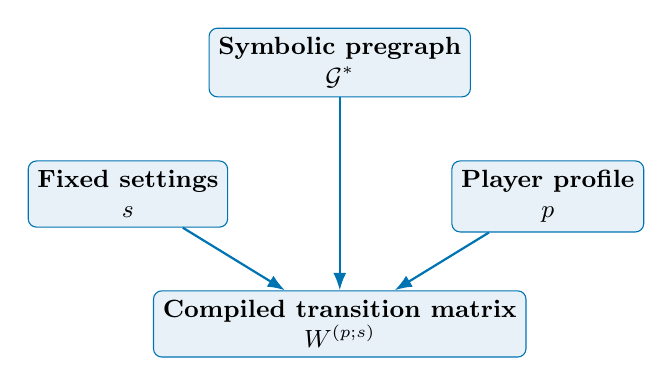
\begin{tikzpicture}[node distance=0.55cm]
        \node[flowbox] (pre) {Symbolic pregraph\\$\mathcal{G}^{\ast}$};
        \node[flowbox,below left=0.8cm and -0.25cm of pre] (settings)
          {Fixed settings\\$s$};
        \node[flowbox,below right=0.8cm and -0.25cm of pre] (profile)
          {Player profile\\$p$};
        \node[flowbox,below=2.45cm of pre,minimum width=4.5cm] (w)
          {Compiled transition matrix\\$W^{(p;s)}$};
        \draw[flowarrow] (pre) -- (w);
        \draw[flowarrow] (settings) -- (w);
        \draw[flowarrow] (profile) -- (w);
      \end{tikzpicture}

      \vspace{2mm}
      \small One reusable pregraph is compiled into all \textbf{27} factorial profiles.

    \column{0.48\textwidth}
      \begin{block}{Affinity and local normalisation}
        \footnotesize
        Each semantic axis contributes a coefficient:
        \begingroup
        \setlength{\abovedisplayskip}{3pt}
        \setlength{\belowdisplayskip}{3pt}
        \[
          r_p(e)=\prod_{a\in\{r,m,c\}} \alpha_a(p,e),
          \qquad
          \alpha\in\{2,1,0.5\}.
        \]
        matching $=2$, neutral $=1$, opposed $=0.5$.
        \[
          W_{ij}^{(p)}=
          \frac{r_p(i,j)}{\sum_k r_p(i,k)},
          \qquad \sum_j W_{ij}^{(p)}=1.
        \]
        \endgroup
      \end{block}
  \end{columns}

  \vspace{1mm}
  \centering\footnotesize
  \textcolor{warncolor}{\textbf{Trajectory probability:}}
  $\displaystyle P(\pi\mid p)=\prod_{(i,j)\in\pi}W_{ij}^{(p)}$.
  Profiles change the story distribution, not the text.
\end{frame}

% Slide 8
\fullslide{graph_neutral_neutral_neutral_slide.png}

% Slide 9
\begin{frame}{Bag-of-Paths aggregates all possible trajectories}
  \begin{columns}[T,onlytextwidth]
    \column{0.42\textwidth}
      \begin{block}{Random-walk BoP boundary}
        \small For the transient block $Q$ of each compiled $W^{(p)}$:
        \[
          N=(I-Q)^{-1}.
        \]
        $N_{si}$ is the expected number of visits to paragraph $i$ from the start $s$.
      \end{block}

      \begin{block}{Analytical, not sampled}
        \small Absorption, visits, edge flows, entropy and conditional quantities are
        computed in closed form for each of the 27 profiles.
      \end{block}

    \column{0.54\textwidth}
      \begin{block}{Three questions}
        \begin{enumerate}
          \item \textbf{Importance:} which passages form the narrative backbone?
          \item \textbf{Danger:} where does expected mortality accumulate?
          \item \textbf{Sensitivity:} where and how do player profiles diverge?
        \end{enumerate}
      \end{block}

      \vspace{2mm}
      \begin{columns}[T,onlytextwidth]
        \column{0.48\textwidth}
          \centering
          \pill{themecolor}{Local indices}\\[2mm]
          \scriptsize paragraphs and edges
        \column{0.48\textwidth}
          \centering
          \pill{goodcolor}{Global indices}\\[2mm]
          \scriptsize complete reading experience
      \end{columns}
  \end{columns}

  \source{Phase 4 uses the Random-Walk limit of the Bag-of-Paths formalism.}
\end{frame}

% Slides 10--12
\fullslide{01_profile_landscape.png}
\fullslide{02_axis_effects.png}
\fullslide{03_local_index_maps.png}

% Slide 13
\begin{frame}{From structural differences to complete stories}
  \begin{columns}[T,onlytextwidth]
    \column{0.50\textwidth}
      \begin{block}{Controlled design}
        \small
        Seven profiles isolate the neutral centre and both extremes of each axis:

        \medskip
        \centering
        \pill{themecolor}{neutral}
        \pill{riskcolor}{cautious}
        \pill{riskcolor}{reckless}\\[2mm]
        \pill{moralitycolor}{selfish}
        \pill{moralitycolor}{noble}
        \pill{actioncolor}{physical}
        \pill{actioncolor}{tactical}

        \medskip
        Each is crossed with \textbf{Win} and \textbf{Death}: $7\times2=14$ cells.
      \end{block}

      \begin{alertblock}{Why not the MAP path?}
        \small The most probable single path favours short stories. We need a central
        observed path, not the shortest likely one.
      \end{alertblock}

    \column{0.46\textwidth}
      \centering
      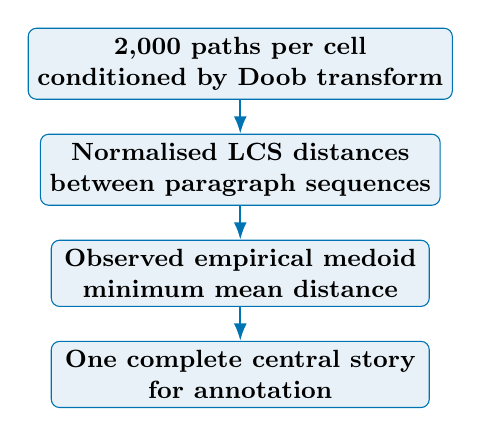
\begin{tikzpicture}[node distance=0.43cm]
        \node[flowbox,minimum width=4.8cm] (sample)
          {2,000 paths per cell\\conditioned by Doob transform};
        \node[flowbox,below=of sample,minimum width=4.8cm] (distance)
          {Normalised LCS distances\\between paragraph sequences};
        \node[flowbox,below=of distance,minimum width=4.8cm] (medoid)
          {Observed empirical medoid\\minimum mean distance};
        \node[flowbox,below=of medoid,minimum width=4.8cm] (story)
          {One complete central story\\for annotation};
        \draw[flowarrow] (sample) -- (distance);
        \draw[flowarrow] (distance) -- (medoid);
        \draw[flowarrow] (medoid) -- (story);
      \end{tikzpicture}
  \end{columns}
\end{frame}

% Slide 14
\begin{frame}{Treating the local LLM as a calibrated instrument}
  \begin{columns}[T,onlytextwidth]
    \column{0.37\textwidth}
      \begin{block}{Qwen3.6-27B receives}
        \small
        \begin{itemize}
          \item complete story text;
          \item eligible player choices;
          \item opaque identifiers;
          \item constrained output schema.
        \end{itemize}
      \end{block}
      \begin{alertblock}{It does not receive}
        \small generator profiles, BoP indices, phase-1 semantic labels or private
        outcome metadata.
      \end{alertblock}

    \column{0.59\textwidth}
      \small
      \begin{tabularx}{\textwidth}{@{}l c X@{}}
        \toprule
        \textbf{Trial} & \textbf{Valid} & \textbf{Objective finding} \\
        \midrule
        P01 & 7/7 & 14 inadmissible mechanical evidence citations \\
        P02 & 5/7 & allow-list helps; two outputs quarantined \\
        P03 & 7/7 & choice/mechanics split; 0 violations \\
        \bottomrule
      \end{tabularx}

      \vspace{4mm}
      \begin{exampleblock}{Freeze before the complete run}
        \small Four individual stories and three pairs were human-annotated for prompt
        calibration. P03 produced \textbf{32 concordances over 44 fields}, with two human
        abstentions. This is \textbf{not accuracy} and not held-out validation.
      \end{exampleblock}

      \centering
      \pill{goodcolor}{P03 frozen} \quad $\longrightarrow$ \quad
      \pill{themecolor}{26 final tasks} \quad $\longrightarrow$ \quad
      \pill{goodcolor}{0 quarantined}
  \end{columns}
\end{frame}

% Slides 15--16
\fullslide{01_individual_trajectories.png}
\fullslide{02_trajectory_comparisons.png}

% Slide 17
\begin{frame}{A reproducible bridge between choices, structure and stories}
  \begin{columns}[T,onlytextwidth]
    \column{0.32\textwidth}
      \begin{block}{What we learned}
        \footnotesize
        \begin{enumerate}
          \setlength{\itemsep}{1pt}
          \item Profiles substantially alter the probabilistic structure.
          \item Their contrasts are usually perceptible in complete stories.
          \item Risk, morality and action are not narratively orthogonal.
        \end{enumerate}
      \end{block}

    \column{0.32\textwidth}
      \begin{alertblock}{Current limits}
        \footnotesize
        \begin{enumerate}
          \setlength{\itemsep}{1pt}
          \item one gamebook;
          \item simplified mechanics and character state;
          \item small human calibration set, without held-out validation.
        \end{enumerate}
      \end{alertblock}

    \column{0.32\textwidth}
      \begin{exampleblock}{Next test}
        \footnotesize Apply the same pipeline and the \textbf{frozen prompt} to LW02.

        \smallskip
        Transfer, rather than further calibration, is the next methodological test.
      \end{exampleblock}
  \end{columns}

  \vspace{2mm}
  \begin{center}
    \small
    The contribution is not an LLM that ``understands'' literature,\\[1mm]
    but an \textbf{auditable pipeline} connecting local choices, probabilistic structure
    and complete narrative experience.
  \end{center}

  \source{Code, prompts, schemas, annotations and derived tables are versioned separately.}
\end{frame}

\end{document}
